\documentclass{article}
\usepackage[utf8]{inputenc}
\usepackage{changepage}
\usepackage{amsmath}
\usepackage{caption}
\usepackage[makeroom]{cancel}
\usepackage{flexisym}
\usepackage{graphicx} 
\usepackage[spanish,es-tabla]{babel}
\usepackage{mathtools}
\usepackage[]{hyperref}
\usepackage{ amssymb }
\usepackage{ mathrsfs }
\usepackage{enumitem}
\usepackage{amsmath}
\usepackage{imakeidx}
\usepackage{float}
\usepackage[useregional]{datetime2}
\allowdisplaybreaks
\title{Taller1Anadec}

\newenvironment{subs}
{\adjustwidth{1em}{0pt}}
{\endadjustwidth}
\usepackage[left=2.1cm, right=2.1cm, top=2.2cm]{geometry}
\begin{document}
\begin{titlepage}
   \begin{center}
       \vspace*{1cm}
        \Huge
       \textbf{Diagnostico de Escalabilidad de sistema de transmisión}
        
       \vspace{0.5cm}
       \Large
        Análisis de Sistemas de Potencia
 
       \vspace{1.5cm}
 
       \textbf{Nicolás Vergara Durán -201513798\\Nestor Alfonso Rodriguez-201514645\\Nicolás Garzón Rodríguez-201511812\\Andrés Nicolás Parra - 201414486}
 
       \vfill
 
       Informe Técnico
 
       \vspace{0.8cm}
 
       
\includegraphics[width=0.4\textwidth]{LogoUniAndes.png}
 
       Departamento de Ingeniería Eléctrica y Electrónica\\
       Universidad de los Andes\\
       Colombia\\
       \today
 
   \end{center}
\end{titlepage}
\tableofcontents
\listoffigures
\listoftables
\newpage
\section*{Resumen Ejecutivo}


A lo largo de este informe se pretende realizar un análisis técnico para diagnosticar el desempeño futuro del sistema IEEE-RTS. Este es un sistema benchmark diseñado por IEEE para análisis de con fiabilidad, el sistema cuenta con dos áreas interconectadas, una de 230 kV y otra de 138 kV. Para este sistema se prevé un crecimiento del 30\% para el año T en la demanda de todas las cargas, con excepción de la demanda de la siderúrgica ANDES para la cual se considerará una ampliación de 25 MW en el año T (con factor de potencia 0,95 en atraso). Para realizar el análisis técnico se tienen en cuenta como criterios de operación  que el voltaje  del sistema, tanto en condición normal como de contingencia N-1, debe encontrarse entre 0,95 p.u. y 1,05 p.u, además el sistema no debe encontrarse en sobrecarga de ninguno de sus componentes. A partir de esos criterios se realizo  un diagnóstico del sistema para el año T, tanto en condición sin contingencias como de contingencias N-1, en la red de transmisión (no se considerarán contingencias de generación, ni refuerzos de red). Se deberá ajustar la generación del despacho OPF del año 0 para el año T, considerando también las siguientes modificaciones en el sistema:

\begin{itemize}
    \item Se instalará un parque eólico de 200 MW (denominado WPP1) con factor de planta de 0,5
    \item Se instalará un parque eólico de 200 MW (denominado WPP2) con factor de planta de 0,4
    \item Se instalará una planta térmica a gas natural (denominada TG1) de 200 MW
    
\end{itemize}


Al realizar el análisis de flujo de carga en condición normal se observo que a pesar de las modificaciones realizadas en la generacional el sistema no es posible suplir el incremento que se presenta en la demanda. A causa de esto, al realizar el flujo de carga óptimo se obtiene como resultado que no todos los generadores operan a su capacidad nominal y que es el nodo slack el encargado de suplir el déficit de demanda, esto operando por encima del valor máximo posible. Posteriormente se realizo el análisis de flujo de carga para el sistema en estado de contingencia N-1. Para este análisis se tuvieron en cuenta contingencias simples de desconexión de lineas o transformadores. En la tabla a continuación de presentan los resultados de los casos en los que el voltaje de operación se encontraba por fuera del rango definido en los criterios de operación



\begin{table}[H]
\caption*{Tabla I. Resultado analisis de contingencias N-1}
\label{Tabla:Resultado analisis de contingencias N-1}
\centering
\begin{tabular}{|c|c|c|c|}
\hline
Voltaje Máximo & Voltaje Mínimo & Nodos en fuera de rango & Linea en Contingencia \\ \hline
1.035          & 0.9409         & 5                       & 1-5                   \\ \hline
1.035          & 0.9088         & 4                       & 2-4                   \\ \hline
1.035          & 0.948          & 6                       & 2-6                   \\ \hline
1.035          & 0.9023         & 3                       & T 3-24                  \\ \hline
1.035          & 0.6275         & 6                       & 6-10                  \\ \hline
1.035          & 0.8342         & 6,8,9                   & 7-8                   \\ \hline
1.035          & 0.9424         & 9                       & T 9-11                  \\ \hline
1.035          & 0.9496         & 6                       & T 10-11                 \\ \hline
1.035          & 0.9215         & 12,25                   & 12-13                 \\ \hline
1.035          & 0.9328         & 5                       & 13-23                 \\ \hline
1.035          & 0.9366         & 3,12,24,25              & 14-16                 \\ \hline
1.035          & 0.8760         & 3,24                    & 15-24                 \\ \hline
1.035          & 0.9443         & 3                       & 28-3                  \\ \hline
\end{tabular}
\end{table}

De los resultados obtenidos se puede observar que el nodo que presenta un nivel de voltaje mas critico es el nodo 6 cuando se da la contingencia de desconexión de la linea 6-10. El nivel del voltaje de este nodo es de 0,6275 p.u, considerablemente fuera del rango de operación definido. Del resto de casos críticos encontrados se puede evidenciar que la mayoría de nodos que se encuentran fuera de rango se encuentran a un nivel de tensión de 138 Kv, esto puede ocurrir debido a la topología de los nodos a este nivel de tensión es radial, mientras que a un voltaje de 230 Kv la topología es anillada y ante contingencias los niveles de tension en los nodos se ajustan al rango permitido


\newpage
\section{Introducción}
El presente documento tiene como objetivo presentar un análisis técnico para el estudio del sistema IEEE-RTS. Este es un sistema benchmark diseñado por IEEE para análisis de fiabilidad, el sistema cuenta con dos áreas interconectadas, una de 230 kV y otra de 138 kV. El objetivo de este informe es el de presentar el análisis técnico para diagnosticar el desempeño futuro de un sistema de potencia. Dentro de este análisis se busca determinar si el sistema cumple con las especificaciones necesarias para el correcto funcionamiento del sistema, tanto en condición normal como en contingencia N-1, para esto se debe garantizar los perfiles de tensión permitidos por la CREG (0,95-1,05 p.u), garantizar la transmisión de potencia en 3878.5 MW y el sistema no debe encontrarse en sobrecarga de ninguno de sus componentes (líneas y transformadores).

\begin{figure}[H]
    \centering
    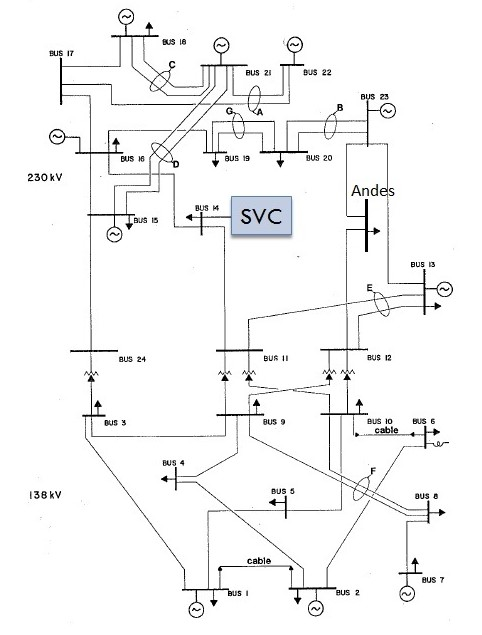
\includegraphics{UnifilarEscenario1.jpg}
    \caption{Conexión Caso base}
    \label{CasoBase}
\end{figure}

\section{Ampliación del sistema de transmisión para el año T}
Con el fin de evaluar la proyección a futuro del sistema en el año T, es necesario realizar un incremento del valor de potencia requerida en las cargas presentes en el sistema, para ello se estimó un aumento del 30\% en cada una de las cargas, a excepción de la carga Andes. En la cual, se presenta un aumento de 25 MW que conserva el factor de potencia en 0.95. Una vez realizada la proyección de la demanda, en función de aumentar la capacidad de generación del sistema se implementaron 2 parques eólicos y una planta térmica conectadas como se presenta en la figura \ref{UnifilarAnoT} :

\begin{figure}[H]
    \centering
    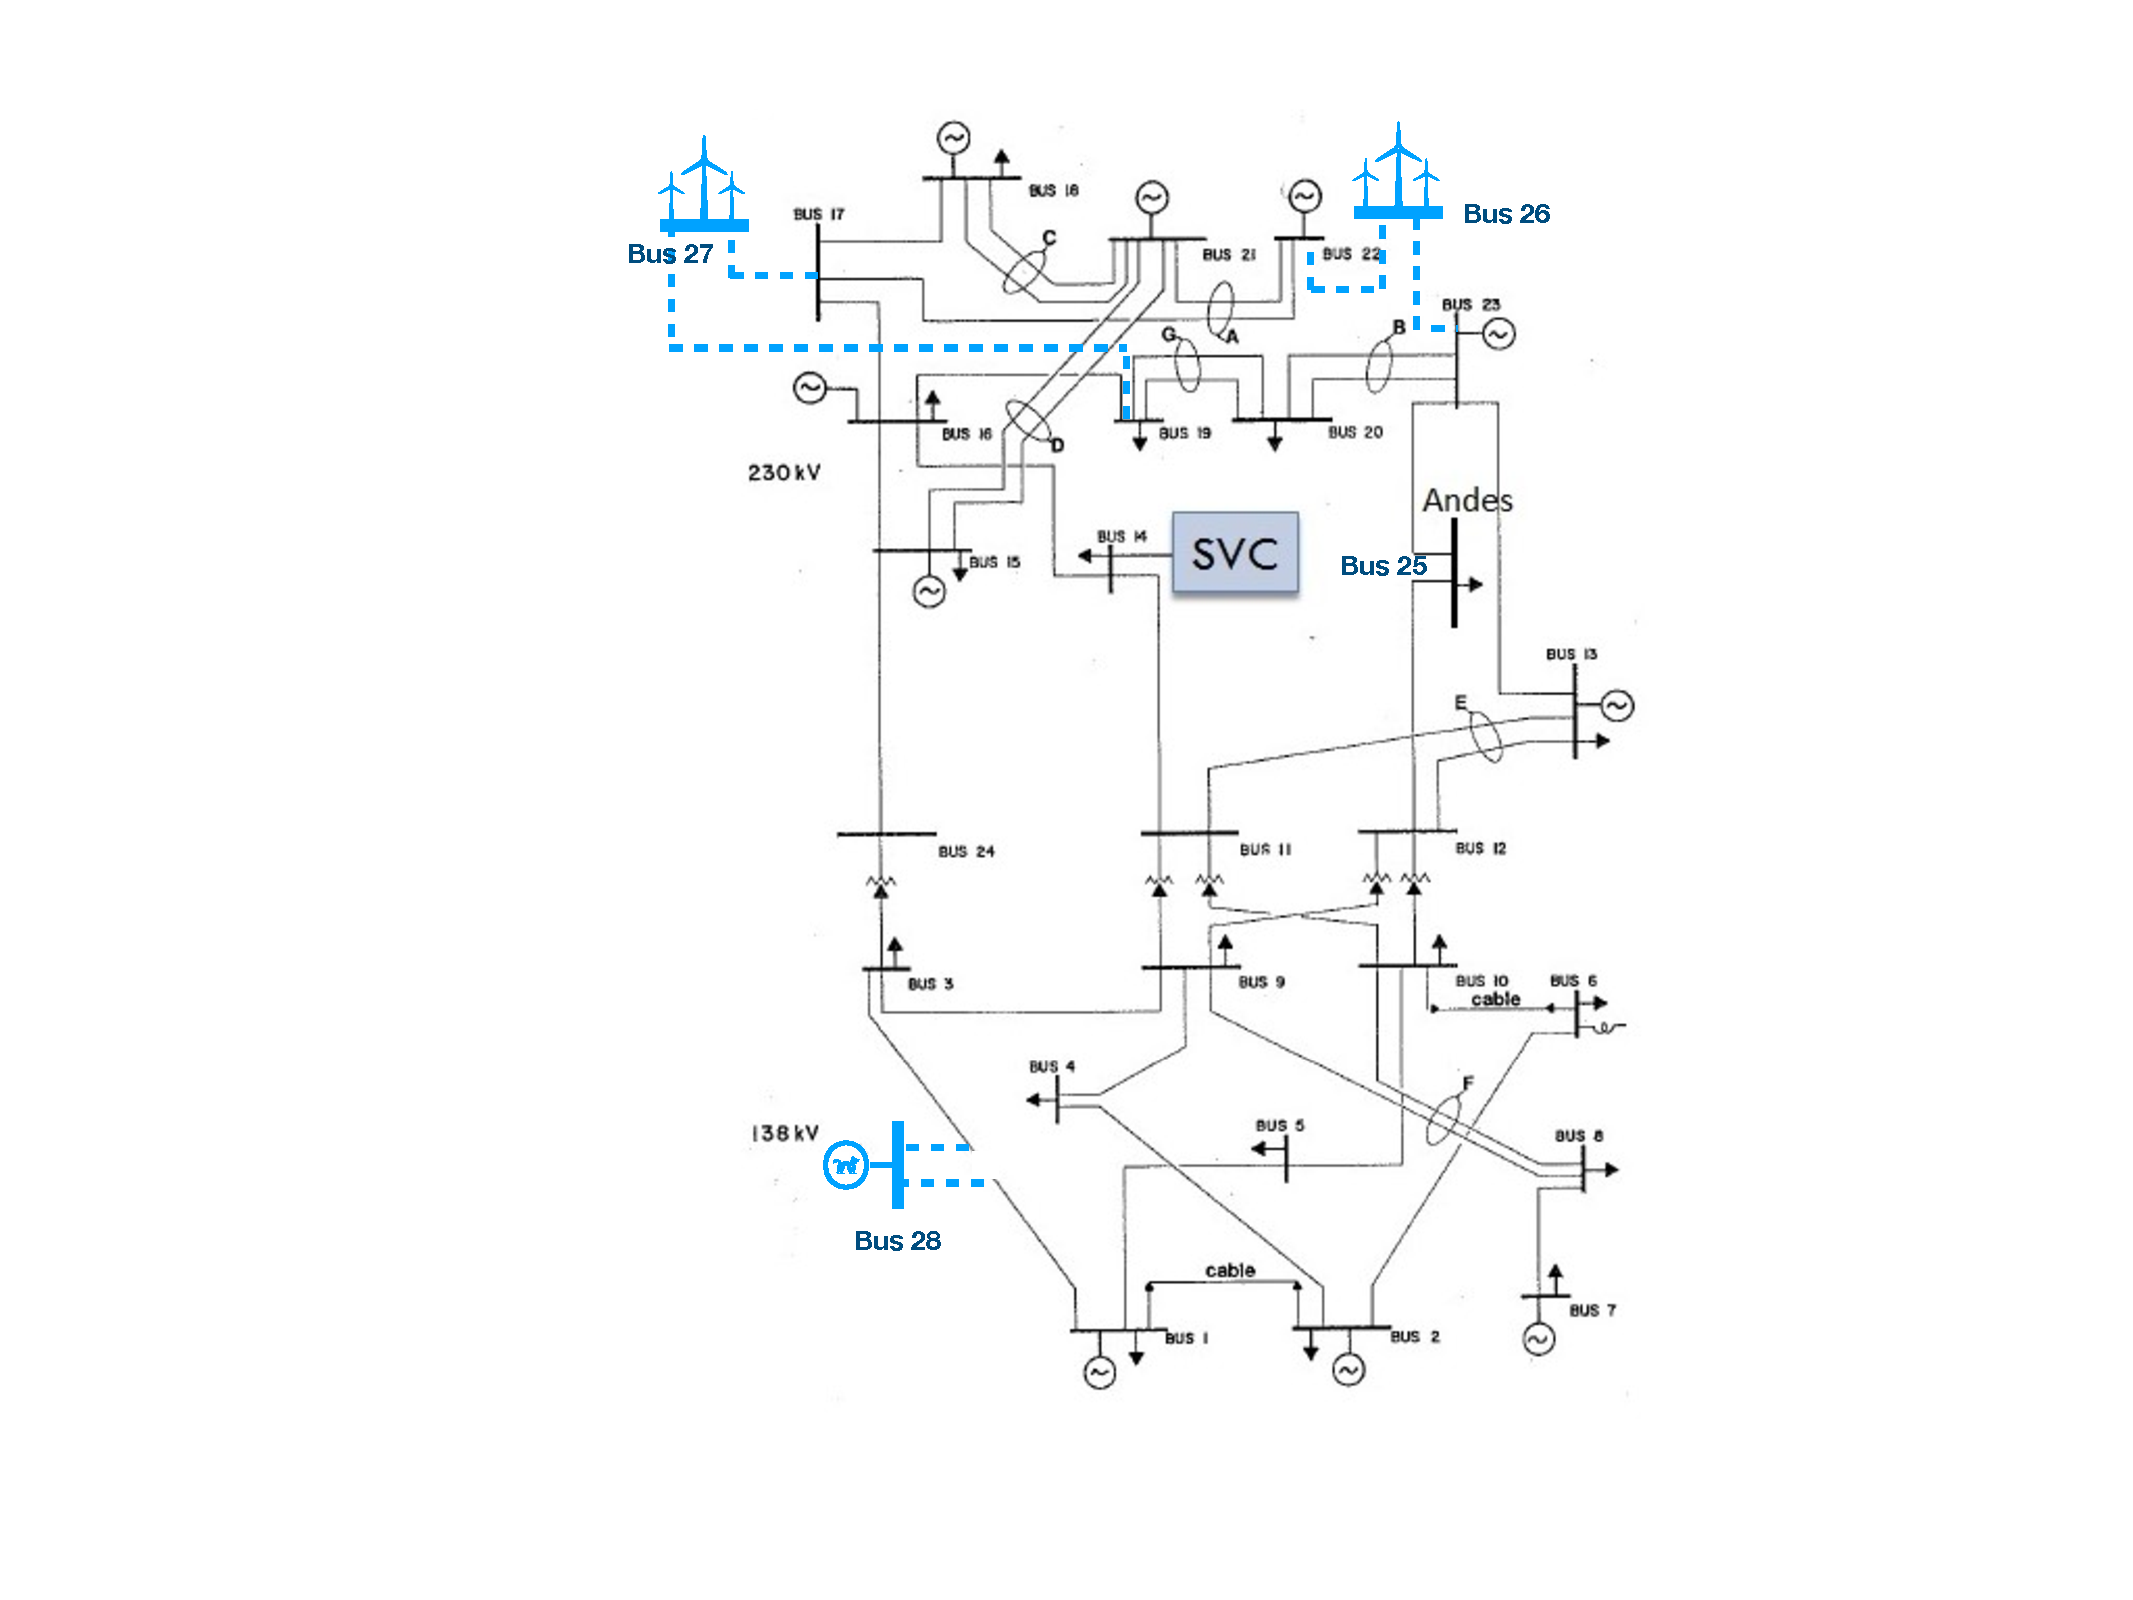
\includegraphics[scale=0.7]{UnifilarDragon.pdf}
    \caption{Diagrama Unifilar de conexión proyectada para el año T}
    \label{UnifilarAnoT}
\end{figure}
A continuación se presenta una descripción de la implementación de los sistemas de generación eléctricos conectados al sistema de transmisión:
\subsection{Plantas Eólicas}
Para la integración adecuada de fuentes no convencionales de energía, es menester garantizar que los limites de generación de potencia establecidos por resolución 060 de 2019 de la CREG, capitulo 5.7 sección B, se cumplan. En esta resolución se establece que el rango operativos de potencia reactiva de una planta eólica debe encontrarse entre 0.33 y -0.33 p.u, cumpliendo así mismo la distribución presentada en la figura \ref{LimitesEolica}.



\begin{figure}[H]
    \centering
    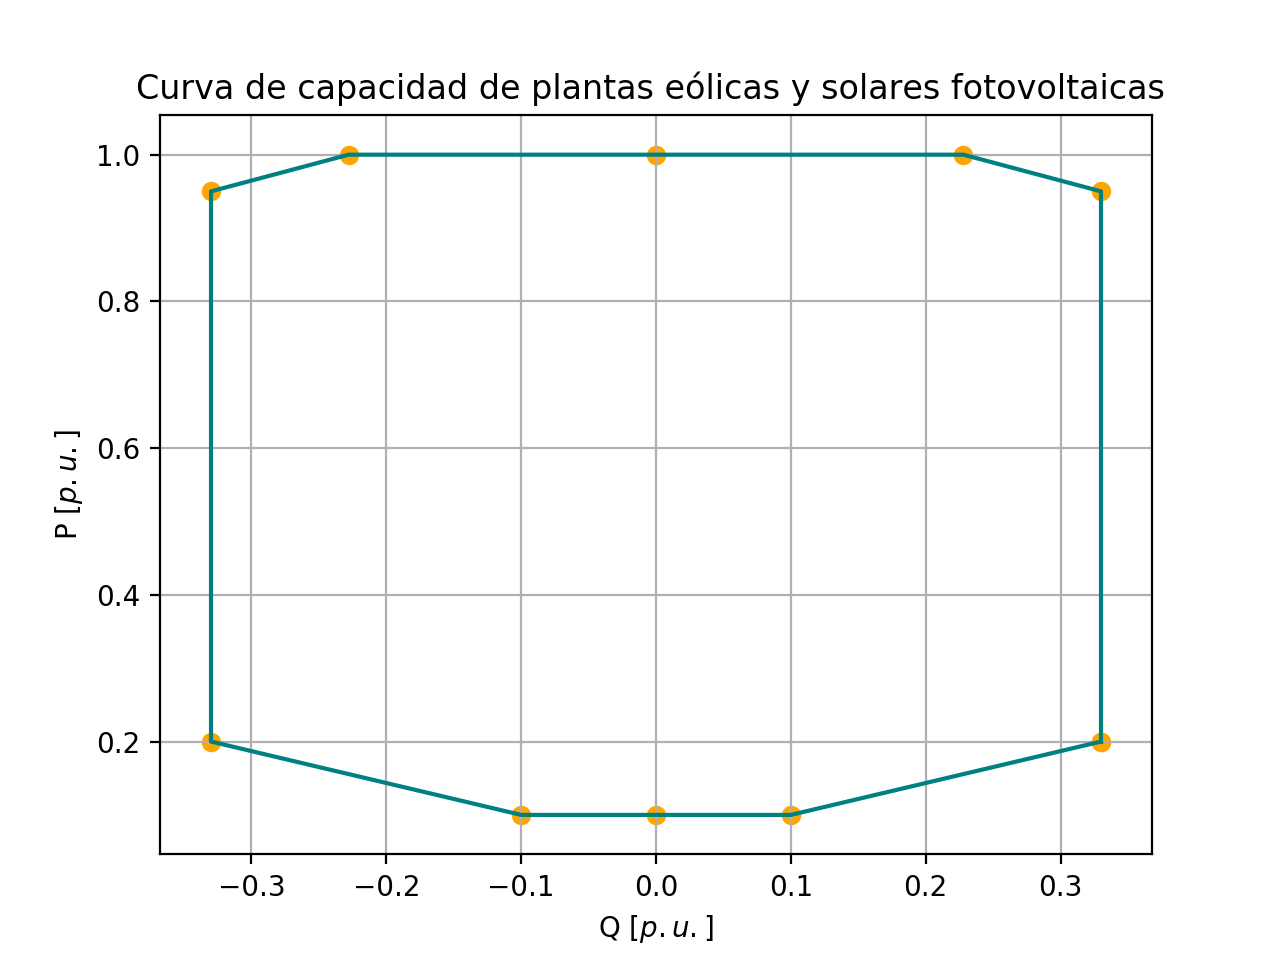
\includegraphics[scale=0.7]{CREG.png}
    \caption{Curva de capacidad de plantas eólicas y solares fotovoltaicas, regulado por resolución 060 de 2019 de la CREG}
    \label{LimitesEolica}
\end{figure}

De igual manera dada la naturaleza de las plantas térmicas, el costo de generación asociado a la planta es $\$0$\footnote{el costo de generación es nulo puesto que, el recurso de generación asociado (aire) es de uso libre. Sin embargo, por esta misma razón no se puede establecer control sobre la generación de la planta debido a que depende totalmente de condiciones ambientales.}. Dadas las limitaciones ambientales se modeló el generador a partir de un factor de planta ($fp$), este es el cociente entre la potencia real generada en la zona y la potencia nominal del generador. $fp=\frac{P_R}{P_N}$  \\

En primera instancia, se proyectó la conexión del parque eólico WPP1, este se estableció en un nuevo bus denominado por el numero 26. Este parque eólico posee una capacidad nominal de generación de 200 $MW$ y un factor de planta $fp=0.5~$. Esta planta se conecta a los buses 22 y 23, cada uno por medio de una linea de $75 km$ y $25km$ respectivamente tal como se muestra en la figura \ref{WPP1}.  
\begin{figure}[H]
    \centering
    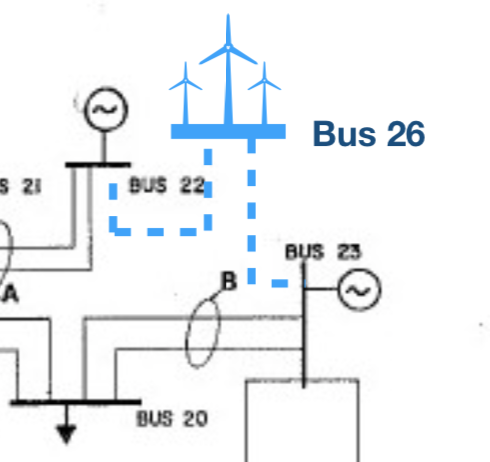
\includegraphics[scale=0.7]{ParqueEolico1.png}
    \caption{Conexión del parque eólico WPP1 al sistema de transmisión}
    \label{WPP1}
\end{figure}
Luego, se proyectó la conexión del parque eólico WPP2, este se estableció en un nuevo bus denominado por el numero 27. Este parque eólico posee una capacidad nominal de generación de 200 $MW$ y un factor de planta $fp=0.4~$. Esta planta se conecta a los buses 17 y 19, cada uno por medio de una linea de $45 km$ y $75km$ respectivamente tal como se muestra en la figura \ref{WPP2}. 
\begin{figure}[H]
    \centering
    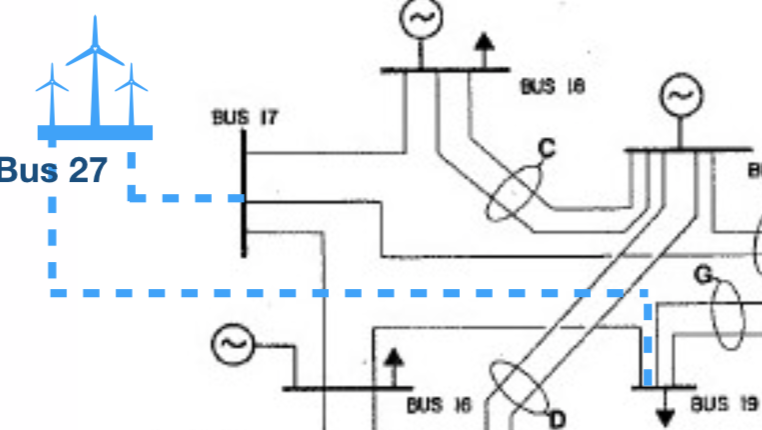
\includegraphics[scale=0.7]{ParqueEolico2.png}
    \caption{Conexión del parque eólico WPP2 al sistema de transmisión}
    \label{WPP2}
\end{figure}
\subsection{Planta térmica a gas natural }
En la sección del sistema de transmisión de $138kV$ se proyectó la conexión de una planta térmica que funciona a partir de gas natural. Esta planta se modeló con una curva de costos de generación cuadrática, cuya expresión esta dada por $$C=212.3076 + 16.0811P +0.014142P^2 $$ .

De igual manera, se debe garantizar que la planta cumpla con los requerimientos de generación de potencia reactiva, es decir un factor de potencia\footnote{el factor de potencia es relación entre la potencia activa P, y la potencia aparente S. $~f.d.p=\frac{P}{S}$} límite de $f.d.p=0.85$ por lo cual se fijó como requerimiento del flujo de carga que la potencia reactiva del generador estuviera limitada a $Q_{max}=123.95 MVar ~\land ~ Q_{min}=-123.95 MVar$. Dado que la potencia nominal del generdor es $P_{nom}=200MW$.\\

Para conectar este generador se abrió la linea que conectaba al bus 1 y 3, así pues se conectó el generador térmico entre estos nodos. Además se denominó el bus de conexión como bus 28. Asimismo para realizar la conexión de la planta se tuvo que, la longitud de la linea para la conexión del bus 28 a los buses 1 y 3 fueron $52km$ y $60km$ respectivamente. 
\begin{figure}[H]
    \centering
    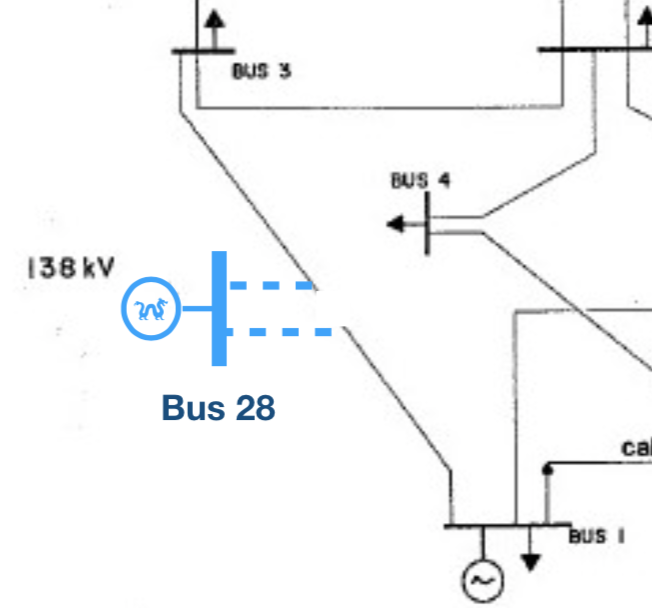
\includegraphics[scale=0.6]{DragonTermico.png}
    \caption{Conexión de la planta térmica a gas natural TG1 al sistema de transmisión}
    \label{TG1}
\end{figure}
\subsection{Cálculo de parámetros de lineas de conexión de los generadores}
Finalmente para realizar el análisis técnico es necesario calcular los valores por unidad de las lineas que se añadieron al sistema de transmisión e incluir estos parámetros en el modelo. Para realizar el calculo de los valores por unidad se determinó primero el calibre del cable para el sistema de tensión \footnote{Para determinar el calibre del cable utilizado en la línea se tomó la impedancia por unidad de otra linea conectada al mismo nivel de tensión. Luego, se halló $Z_{Base}$ y luego con la longitud de la línea se calculó la resistividad por unidad de longitud. $ R[\frac{\Omega}{Km}]=\frac{R_{p.u.}Z_{base}}{longitud}$} de tal forma que para el nivel de tensión de $230kV$ cable ACSR Canary de $900kcmil$ y $138kV$cable ACSR Patridge de $266.8kcmil$. A continuación se calculó la resistividad total con la distancia y luego se convirtió el valor por unidad. Finalmente se tomaron valores típicos para el nivel de tensión para la reactancia y la susceptancia en función de la resistencia. A partir de los cálculos efectuados en el script de matlab  se obtuvo los valores presentados en la tabla \ref{parametros}.

\begin{table}[H]
\centering
\caption{Parámetros por unidad de lineas agregadas al sistema.}
\label{parametros}
\resizebox{0.5\textwidth}{!}{%
\begin{tabular}{|c|c|c|c|c|}
\hline
Nodo 1 & Nodo 2 & R p.u & X p.u. & B p.u. \\ \hline
26 & 22 & 0.0090 & 0.0898 & 0.2806 \\ \hline
26 & 23 & 0.0030 & 0.0299 & 0.0935 \\ \hline
27 & 17 & 0.0054 & 0.0539 & 0.1684 \\ \hline
27 & 19 & 0.0090 & 0.0898 & 0.2806 \\ \hline
28 & 3 & 0.0370 & 0.1432 & 0.0388 \\ \hline
28 & 1 & 0.0321 & 0.1241 & 0.0336 \\ \hline
\end{tabular}%
}
\end{table}
\newpage




\section{Análisis técnico}

Se realizo el diagnostico del sistema tanto normal como en estado de contingencia N-1 teniendo en cuenta los siguientes criterios: 
\begin{itemize}
    \item Los perfiles de voltaje se deben encontrar entre 0.95 y 1.05 p.u
    \item No se deben presentar elementos sobrecargados ( lineas y transformadores)
    \item Se debe garantizar el suministro de potencia a las cargas
\end{itemize}

Como herramienta para realizar el diagnostico se utilizo el software Matpower, dadas las condiciones del software utilizado, se establecieron los limites de los elementos de manera que no se encontraran en sobrecarga. Posteriormente, se realizo la proyección del crecimiento de la carga al año T, la cual corresponde a un incremento de 30 en todos los nodos de carga, a excepción del nodo 25 correspondiente a la carga "ANDES", la cual presenta un incremento de 25MW a factor de potencia 0.95. En seguida, se puede observar en la tabla \ref{Demandas} la potencia demandada en cada nodo. 




Se puede observar un incremento de la demanda total del sistema de 2968.1MW a 3878.5 MW, lo que indica que la demanda total disponible de generación 3780MW no es suficiente para suplir los requerimientos del sistema, estos resultados se pueden comprobar a través del anexo electrónico case24\_Escenario1.m y ExpansionT.m, en la sección bus data.

\subsection{Análisis en condición normal}

Inicialmente, se realizo un análisis de flujo de carga en condiciones operativas normales, esto con el fin de establecer el adecuado funcionamiento del sistema, a partir de este análisis fue posible observar que las adiciones de los generadores no son suficientes para suplir el incremento de la demanda. A causa de esto se pudo observar que los resultados obtenidos utilizando el modelo de flujo de carga óptimo, no indica que todos los generadores están operando a su capacidad nominal, siendo el generador slack el encargado de suplir el déficit de demanda operando por encima de su valor máximo, para el caso presentado este corresponde al nodo 23. \\

Se estableció el voltaje de operación de los generadores en 1.03PU, con el fin de que estos evitaran la caída de tensión producida debido a el incremento en la demanda, se observo que todos los voltajes se encuentran dentro de los rangos permitidos por la regulación de la CREG, los voltajes son presentados en la tabla \ref{CondicionesNormales}.



Se identifico que el caso de condiciones de operación normales no  cumple con las condiciones establecidas, no se encontraron elementos en sobrecarga, ni nodos con sobre-tensión, sin embargo, no se logra se suplir la demanda de manera adecuada con la capacidad de generación disponible, esto se evidencia en que el nodo slack esta supliendo potencia en un valor superior a sus limites operativos. Estos resultados se obtuvieron usando la herramienta matpower mediante el código ExpansionAnioT.m. 

\newpage
\subsection{Análisis de contingencias N-1}

Posteriormente se realizo el análisis del sistema en estado de contingencia N-1, se tomaron en cuenta contingencias simples de desconexión de lineas y desconexión de transformadores.  A continuación se presentan los resultados para los casos crítico  en los que los voltajes de los nodos se encuentran por fuera del rango de 0.95 - 1.05 p.u


\begin{table}[H]
\centering
\caption{Líneas que no cumplen análisis de contingencias para el año T}
\begin{tabular}{|c|c|c|c|}
\hline
Voltaje Máximo & Voltaje Mínimo & Nodos en fuera de rango & Linea en Contingencia \\ \hline
1.035          & 0.9409         & 5                       & 1-5                   \\ \hline
1.035          & 0.9088         & 4                       & 2-4                   \\ \hline
1.035          & 0.948          & 6                       & 2-6                   \\ \hline
1.035          & 0.9023         & 3                       & T 3-24                  \\ \hline
1.035          & 0.6275         & 6                       & 6-10                  \\ \hline
1.035          & 0.8342         & 6,8,9                   & 7-8                   \\ \hline
1.035          & 0.9424         & 9                       & T 9-11                  \\ \hline
1.035          & 0.9496         & 6                       & T 10-11                 \\ \hline
1.035          & 0.9215         & 12,25                   & 12-13                 \\ \hline
1.035          & 0.9328         & 5                       & 13-23                 \\ \hline
1.035          & 0.9366         & 3,12,24,25              & 14-16                 \\ \hline
1.035          & 0.8760         & 3,24                    & 15-24                 \\ \hline
1.035          & 0.9443         & 3                       & 28-3                  \\ \hline
\end{tabular}
\end{table}
En nodo fuera de rango más critico del sistema es el nodo 6 al desconectar la línea 6-10.El generador del nodo 13, el cual se conecta directamente en el transformador T10-11,y este a su ves, se conecta al nodo 10, suple potencia a la carga del nodo 6 donde no converge, debido a que en el nodo 6 el perfil de tensión mínimo cae a un nivel de 0.627 pu, el cual esta considerablemente por fuera de rango permitido por la CREG.En general, la mayoría de los nodos que están fuera de rango permitido son los que están al nivel de tensión de 138 kV, debido a que la topología es más radial que los nodos que se conectan a 230, en donde la topología es mas anillada y ante contingencias,los niveles de tensión dentro procuran estar dentro del rango permitido.
\begin{table}[H]
\centering
\caption{Perdidas del }
\begin{tabular}{|c|c|c|c|}
\hline
Año & Ploss(MW) & Qloss (MVAr)  \\ \hline
0                       & 71.80                         & 541.31                         \\\hline
T                       & 98.52                         & 819.93                        \\\hline
\end{tabular}
\end{table}
La tabla anterior muestra el nivel de perdías para el caso base en el año 0  y el caso en el año T, donde fueron incluidas las nuevas fuentes de generación. Al la potencia generada, aumentan las perdidas de potencia activa y reactiva en el sistema considerablemente, debido a que ante contingencia N-1, los generadores carecen de la capacidad de soporte del sistema y se deben  mantener los niveles de tensión en los nodos y en las ramas, dentro de los límites establecidos.
\section{Conclusiones}

\begin{itemize}
    \item Se identifico que la potencia requerida en el año T, no puede ser suministrada mediante los generadores presentes en el sistema, dado que estos no tienen la capacidad suficiente para suplir la demanda.
    
    \item Se encontró que los nodos con mayor incidencia a presentar caídas de tensión por fuera de los rangos de operación, son los nodos 3, 6 y 9, los cuales se encuentran todos operando a 138kV, por lo que se recomiendan refuerzos a este nivel de tensión.
    
    \item Se observo que el nodo 7 no cumple con el criterio N-1, por lo que se recomienda un refuerzo posterior sobre este nodo.
    
    \item Se observo que el caso critico corresponde a la contingencia en la linea 6-10, puesto que la salida de servicio de esta linea causa que el voltaje del nodo 6 caiga al valor de 0.6275 p.u, se requiere un refuerzo sobre este elemento.
    
    \item Se observa un incremento significativo en las perdidas, esto puede ser causado debido a que al no cumplirse con la demanda de generación, el slack suple esta demanda, causando que hayan grandes flujos de corriente sobre algunos elementos del sistema.
\end{itemize}

\section{Anexos}
\begin{table}[H]
\centering
\caption{Demandas del sistema en el año 0 y en el año T }
\begin{tabular}{|c|c|c|c|c|}
\hline


Bus & \multicolumn{2}{c|}{Caso Base} & \multicolumn{2}{c|}{Año t} \\ \hline
\#  & P(MW)         & Q(MVar)        & P(MW)       & Q(MVar)      \\ \hline
1   & 108           & 22             & 140.4       & 28.6         \\ \hline
2   & 97            & 20             & 126.1       & 26           \\ \hline
3   & 180           & 37             & 234         & 48.1         \\ \hline
4   & 74            & 15             & 96.2        & 19.5         \\ \hline
5   & 71            & 14             & 92.3        & 18.2         \\ \hline
6   & 136           & 28             & 176.8       & 36.4         \\ \hline
7   & 125           & 25             & 162.5       & 32.5         \\ \hline
8   & 171           & 35             & 222.3       & 45.5         \\ \hline
9   & 175           & 36             & 227.5       & 46.8         \\ \hline
10  & 195           & 40             & 253.5       & 52           \\ \hline
11  & 0             & 0              & 0           & 0            \\ \hline
12  & 0             & 0              & 0           & 0            \\ \hline
13  & 265           & 54             & 344.5       & 70.2         \\ \hline
14  & 194           & 39             & 252.2       & 50.7         \\ \hline
15  & 317           & 64             & 412.1       & 83.2         \\ \hline
16  & 100           & 20             & 130         & 26           \\ \hline
17  & 0             & 0              & 0           & 0            \\ \hline
18  & 333           & 68             & 432.9       & 88.4         \\ \hline
19  & 181           & 37             & 235.3       & 48.1         \\ \hline
20  & 128           & 26             & 166.4       & 33.8         \\ \hline
21  & 0             & 0              & 0           & 0            \\ \hline
22  & 0             & 0              & 0           & 0            \\ \hline
23  & 0             & 0              & 0           & 0            \\ \hline
24  & 0             & 0              & 0           & 0            \\ \hline
25  & 50            & 16.434         & 75          & 24.6514      \\ \hline
26  & 0             & 0              & 0           & 0            \\ \hline
27  & 0             & 0              & 0           & 0            \\ \hline
28  & 0             & 0              & 0           & 0            \\ \hline

\end{tabular}
\label{Demandas}
\end{table}

\begin{table}[H]
\centering
\caption{Resultados flujo de carga condiciones normales de operación}
\label{CondicionesNormales}
\begin{tabular}{|c|c|c|c|c|c|}
\hline
\textbf{Bus} & Voltaje & \multicolumn{2}{c|}{Generación} & \multicolumn{2}{c|}{Carga} \\ \hline
\textbf{\#}  & (P.U)   & MW              & MVar          & MW           & MVar        \\ \hline
\textbf{1}   & 1.035   & 172.00          & 162.62        & 140.40       & 28.60       \\ \hline
\textbf{2}   & 1.020   & 172.00          & -65.65        & 126.10       & 26.00       \\ \hline
\textbf{3}   & 0.978   & -               & -             & 234.00       & 48.10       \\ \hline
\textbf{4}   & 0.974   & -               & -             & 96.20        & 19.50       \\ \hline
\textbf{5}   & 1.002   & -               & -             & 92.30        & 18.20       \\ \hline
\textbf{6}   & 0.980   & -               & -             & 176.80       & 36.40       \\ \hline
\textbf{7}   & 1.030   & 240.00          & 104.63        & 162.50       & 32.50       \\ \hline
\textbf{8}   & 0.975   & -               & -             & 222.30       & 45.50       \\ \hline
\textbf{9}   & 0.983   & -               & -             & 227.50       & 46.80       \\ \hline
\textbf{10}  & 1.005   & -               & -             & 253.50       & 52.00       \\ \hline
\textbf{11}  & 0.999   & -               & -             & -            & -           \\ \hline
\textbf{12}  & 0.977   & -               & -             & -            & -           \\ \hline
\textbf{13}  & 1.030   & 285.30          & 314.30        & 344.50       & 70.20       \\ \hline
\textbf{14}  & 1.030   & 0.00            & 195.80        & 252.20       & 50.70       \\ \hline
\textbf{15}  & 1.030   & 215.00          & 215.02        & 412.10       & 83.20       \\ \hline
\textbf{16}  & 1.030   & 155.00          & 105.91        & 130.00       & 26.00       \\ \hline
\textbf{17}  & 1.031   & -               & -             & -            & -           \\ \hline
\textbf{18}  & 1.030   & 400.00          & 83.69         & 432.90       & 88.40       \\ \hline
\textbf{19}  & 1.020   & -               & -             & 235.30       & 48.10       \\ \hline
\textbf{20}  & 1.022   & -               & -             & 166.40       & 33.80       \\ \hline
\textbf{21}  & 1.030   & 400.00          & -45.48        & -            & -           \\ \hline
\textbf{22}  & 1.030   & 300.00          & -55.68        & -            & -           \\ \hline
\textbf{23}  & 1.030   & 1159.22         & 101.53        & -            & -           \\ \hline
\textbf{24}  & 0.983   & -               & -             & -            & -           \\ \hline
\textbf{25}  & 0.976   & -               & -             & 75.00        & 24.65       \\ \hline
\textbf{26}  & 1.030   & 100.00          & -28.18        & -            & -           \\ \hline
\textbf{27}           & 1.030   & 80.00           & -19.65        & -            & -           \\ \hline
\textbf{28}           & 1.035   & 200.00          & -0.75         & -            & -           \\ \hline
\end{tabular}
\end{table}



\begin{table}[H]
\centering
\caption{Resultados flujo de carga para año T}
\label{flujo 2}
\resizebox{0.5\textwidth}{!}{%
\begin{tabular}{|l|c|c|r|r|r|r|}
\hline
\multicolumn{1}{|c|}{Bus} & \multicolumn{2}{c|}{Voltaje} & \multicolumn{2}{c|}{Generación} & \multicolumn{2}{c|}{Load} \\ \hline
\multicolumn{1}{|c|}{\#} & Mag (pu) & Ang (deg & \multicolumn{1}{c|}{P (MW)} & \multicolumn{1}{c|}{Q (MVAr)} & \multicolumn{1}{c|}{P (MW)} & \multicolumn{1}{c|}{Q (MVAr)} \\ \hline
1 & -0.035 & 30.28 & 172 & 162.62 & 140.4 & 28.6 \\ \hline
2 & 1.02 & -30.656 & 172 & -65.65 & 126.1 & 26 \\ \hline
3 & 0.978 & -26.693 & - & - & 234 & 48.1 \\ \hline
4 & 0.974 & -33.752 & - & - & 96.2 & 19.5 \\ \hline
5 & 1.002 & -34.047 & - & - & 92.3 & 18.2 \\ \hline
6 & 0.98 & -37.586 & - & - & 176.8 & 36.4 \\ \hline
7 & 1.03 & -37.635 & 240 & 104.63 & 162.5 & 32.5 \\ \hline
8 & 0.975 & -39.688 & - & - & 222.3 & 45.5 \\ \hline
9 & 0.983 & -30.672 & - & - & 227.5 & 46.8 \\ \hline
10 & 1.005 & -33.669 & - & - & 253.5 & 52 \\ \hline
11 & 0.999 & -23.184 & - & - & - & - \\ \hline
12 & 0.977 & -22.182 & - & - & - & - \\ \hline
13 & 1.03 & -18.671 & 285.3 & 314.3 & 344.5 & 70.2 \\ \hline
14 & 1.03 & -18.902 & 0 & 195.8 & 252.2 & 50.7 \\ \hline
15 & 1.03 & -9.321 & 215 & 215.02 & 412.1 & 83.2 \\ \hline
16 & 1.03 & -9.281 & 155 & 105.91 & 130 & 26 \\ \hline
17 & 1.031 & -5.522 & - & - & - & - \\ \hline
18 & 1.03 & -4.694 & 400 & 83.69 & 432.9 & 88.4 \\ \hline
19 & 1.02 & -7.034 & - & - & 235.3 & 48.1 \\ \hline
20 & 1.022 & -3.092 & - & - & 166.4 & 33.8 \\ \hline
21 & 1.03 & -3.716 & 400 & -45.48 & - & - \\ \hline
22 & 1.03 & 2.153 & 300 & -55.68 & - & - \\ \hline
23 & 1.03 & 0 & *  1159.22 & 101.53 & - & - \\ \hline
24 & 0.983 & -15.519 & - & - & - & - \\ \hline
25 & 0.976 & -12.896 & - & - & 75 & 24.65 \\ \hline
26 & 1.03 & 1.76 & 100 & -28.18 & - & - \\ \hline
27 & 1.03 & -4.633 & 80 & -19.65 & - & - \\ \hline
28 & 1.035 & -21.372 & 200 & -0.75 & - & - \\ \hline
\end{tabular}%
}
\end{table}
\end{document}
